\section{Results}
% Structure with subsections
% Use of figures / tables (max. 5)
% General description of the results
\subsection{Differentially Expressed Genes and Network creation}
\begin{itemize}
	\item 908 differentially expressed genes with chosen thresholds section \ref{sec:methods-deg}
	\item around half are upregulated, around half downregulated [TODO: get exact numbers]
	\item String was able to query 828 of them [TODO: provide table of not queried in supplementary material or at least github?]
	\item after querying additional genes that are known to be related to other eds types: resulting network with 847 nodes and 6129 edges
	\item position of known eds genes in network is mostly central (checked degree, clustering coefficient, betweenness centrality and closeness centrality)
\end{itemize}

\subsection{Enrichment analysis and clustering}

\subsubsection{MCODE}

\begin{itemize}
	\item 3 clusters with more than 15 nodes (first with 66 nodes \& 1953 connections, second with 44 nodes \& 686 connections, third with 16 nodes \& 114 connections)
	\item first and largest cluster upregulated only
	\item second one as well
	\item 3rd MCODE cluster, shown in figure \ref{fig:mcode3}, is mostly upgregulated with 2 downregulated nodes, some not relevantly differentially expressed, also only 9/16 are not known eds genes, 8 are
	\item the eds genes are all below the threshold of $|\text{log2FoldChange}| > 0.5$, 1 of them is 1 of the two downregulated genes
	\item quite interesting to see genes closely related to other eds genes, COL21A1 is also strongly upregulated ($\text{log2FoldChange} > 2$)
	\item all known EDS genes with ADAMTS2 as exception have a high Closeness Centrality
	\item regarding the enrichment of this cluster: not surprising to see extracellular
\end{itemize}

\begin{figure}[htb!]
	\centering
	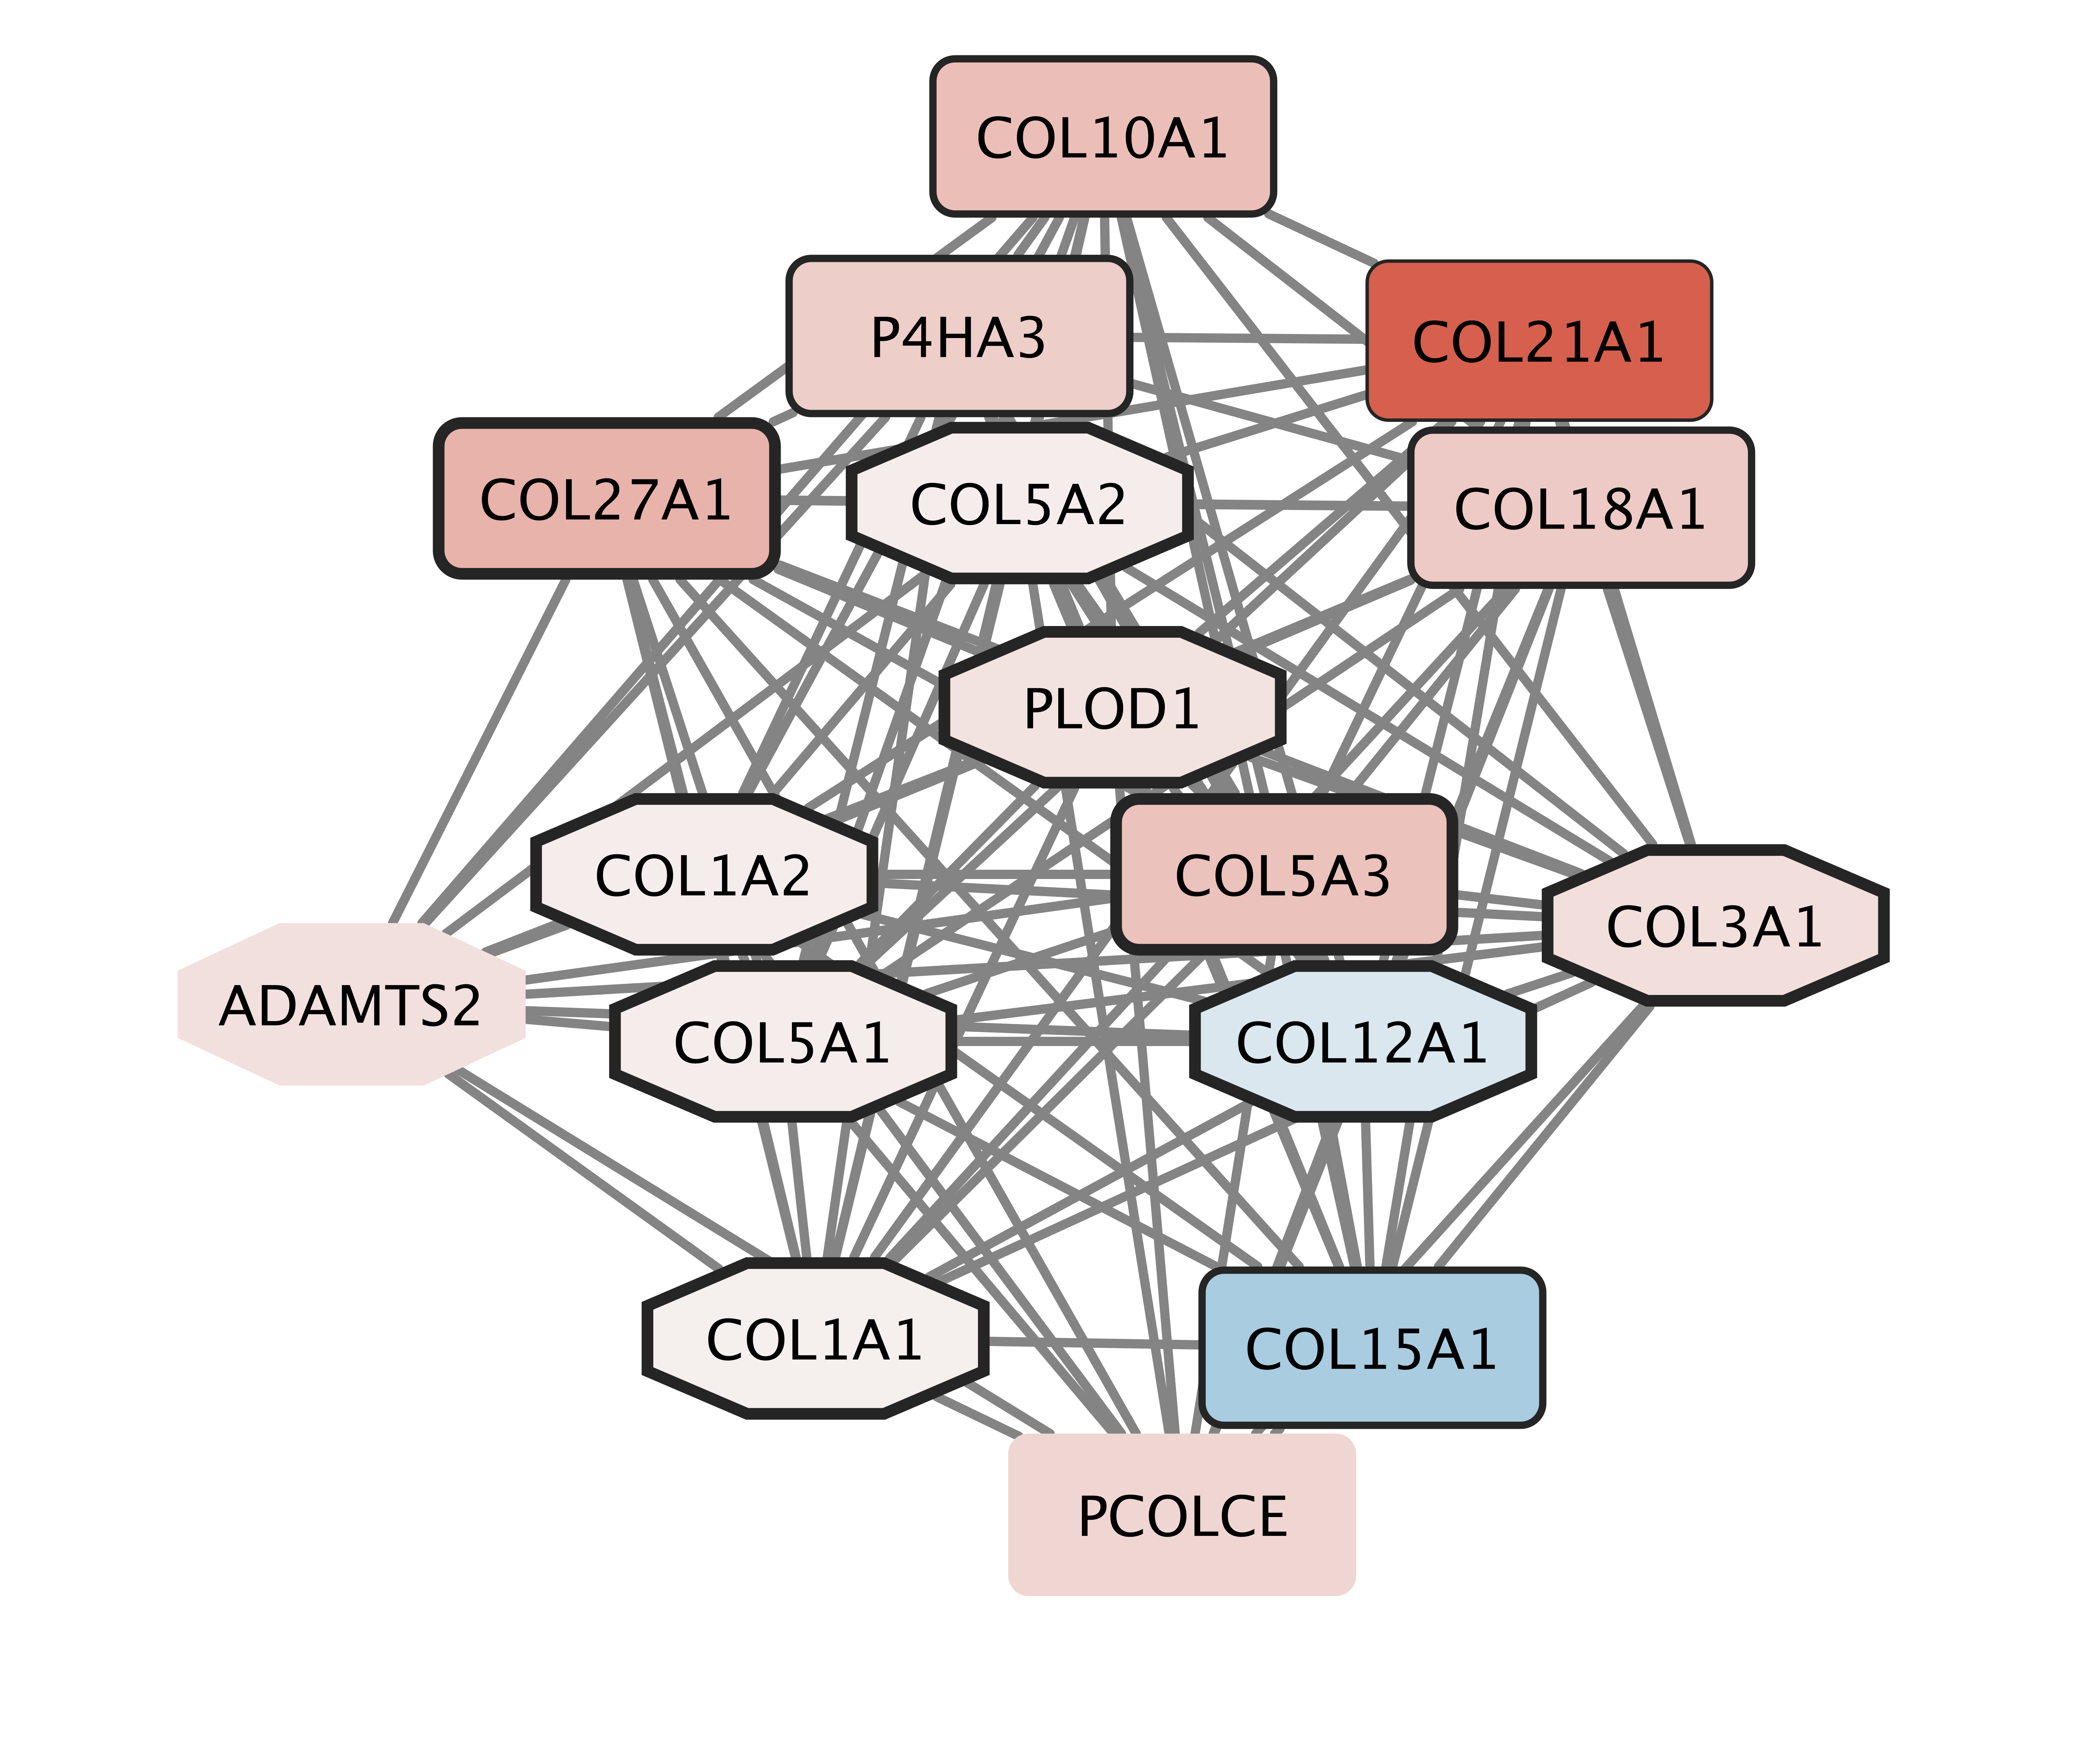
\includegraphics[width=0.6\textwidth]{fig/MCODE-cluster3.png}
	\caption{MCODE cluster 3 [TODO: add legend for shape and colour]}
	\label{fig:mcode3}
\end{figure}

\subsubsection{Community Clustering}

\begin{itemize}
	\item 6 clusters with more than 15 nodes
	\item 3 very small (18, 29, 29 nodes), two medium sized (76 and 105 nodes) and one very large cluster (363 nodes)
	\item especially medium sized clusters highly interconnected
	\item biggest one mix of up-regulated and down-regulated genes, contains all 21 genes known to cause other EDS types
	\item both medium sized clusters mostly upregulated $\rightarrow$ interesting!
\end{itemize}